\documentclass[conference,10pt,a4paper]{IEEEtran}
\usepackage{xeCJK}
\IfFontExistsTF{Times New Roman}{\setmainfont{Times New Roman}}{\setmainfont{texgyretermes-regular.otf}[BoldFont=texgyretermes-bold.otf,ItalicFont=texgyretermes-italic.otf,BoldItalicFont=texgyretermes-bolditalic.otf]}
\IfFontExistsTF{Noto Serif CJK SC}{\setCJKmainfont{Noto Serif CJK SC}[AutoFakeBold=2]}{\IfFontExistsTF{SimSun}{\setCJKmainfont{SimSun}[AutoFakeBold=2]}{\setCJKmainfont{FandolSong-Regular.otf}[BoldFont=FandolSong-Bold.otf]}}
\usepackage{amsmath,amssymb,graphicx,booktabs,array}
\graphicspath{{figures/}}
\providecommand{\ReportAuthors}{作者姓名\enspace\rule{3.2em}{.35pt}\quad 学号\enspace\rule{4.2em}{.35pt}}
\providecommand{\Contribution}{作者排序与贡献\enspace\rule{14em}{.35pt}}
\IfFileExists{authors.tex}{\input{authors.tex}}{}
\newcommand{\SevereRows}{%
纯相机 & 1.38 & 3.84 & 0.75 & 3.17 \\
直接合并雷达框 & 1.09 & 3.00 & 0.65 & 5.13 \\
同型纯图像精修 & 1.91 & 5.56 & 0.90 & 5.51 \\
雷达候选补检＋图像精修 & 2.54 & 8.01 & 0.98 & 11.28 \\
雷达补检（半数帧缺雷达） & 1.93 & 5.73 & 0.90 & 7.33 \\
}
\newcommand{\ClassRows}{%
纯相机 & 3.77 & 0.39 & 0.00 \\
直接合并雷达框 & 2.83 & 0.43 & 0.00 \\
同型纯图像精修 & 5.20 & 0.54 & 0.00 \\
雷达候选补检＋图像精修 & 6.52 & 1.10 & 0.00 \\
雷达补检（半数帧缺雷达） & 4.98 & 0.80 & 0.00 \\
}
\newcommand{\SeedRows}{%
纯相机 & 1.72 & 1.02 & 1.41 & $1.38\pm0.36$ \\
同型纯图像精修 & 2.31 & 1.47 & 1.96 & $1.91\pm0.42$ \\
雷达候选补检＋图像精修 & 3.00 & 2.32 & 2.29 & $2.54\pm0.40$ \\
}

\newcommand{\AbstractResult}{三个随机种子的平均结果表明，雷达补检将纯相机的 mAP50--95 从 1.38\% 提高到 2.54\%，AP50 从 3.84\% 提高到 8.01\%，也超过同型纯图像精修的 1.91\% 和 5.56\%。}
\newcommand{\MainResult}{在表\ref{tab:main}中，雷达补检在强模糊验证集上的 mAP50--95 为 2.54\%，比纯相机、同型纯图像精修及直接合并雷达框分别高 1.16、0.63 和 1.45 个百分点。与纯相机相比，AP50 由 3.84\% 提高至 8.01\%，AR100 由 3.17\% 提高至 11.28\%。表\ref{tab:seeds}和图\ref{fig:diagnostics}给出三个种子的结果。三次运行中，雷达补检的 mAP50--95 均高于纯相机和同型纯图像精修，显示收益方向在当前固定划分上保持一致。}
\newcommand{\DiagnosticResult}{表\ref{tab:classes}显示，相对纯相机，汽车 AP 由 3.77\% 升至 6.52\%，行人 AP 由 0.39\% 升至 1.10\%，自行车 AP 仍为零。整体改善主要来自汽车和行人。移除约一半验证帧的雷达候选后，同一补检器的 mAP50--95 从 2.54\% 降至 1.93\%，AP50 从 8.01\% 降至 5.73\%。在视觉输入保持相同的情况下，这一变化反映补检模型依赖雷达候选来恢复部分检测。}
\newcommand{\ConclusionResult}{在人工高斯强模糊下，基于雷达的独立候选经图像精修后改善了道路目标的二维检测。相对冻结的纯相机基线，三次运行的平均 mAP50--95 提高 1.16 个百分点，AP50 提高 4.17 个百分点。与同型纯图像精修相比，平均 mAP50--95 高 0.63 个百分点。部分雷达缺失时收益减小。}

\newcommand{\ExpansionRows}{%
纯相机 & 1.44 & 3.67 & 1.46 & 3.61 \\
直接合并雷达框 & 1.17 & 2.87 & 1.14 & 2.50 \\
同型纯图像精修 & 2.09 & 5.50 & 2.31 & 6.85 \\
雷达候选补检＋图像精修 & 2.53 & 7.35 & 3.20 & 10.27 \\
雷达补检（半数帧缺雷达） & 1.91 & 5.31 & 2.30 & 6.82 \\
}

\newcommand{\ExpansionAbstract}{冻结权重后，在 30 个未见 nuScenes 场景上，mAP50--95 从 1.44\% 提高到 2.53\%。在独立的 Astyx 数据上，汽车 AP50--95 从 1.46\% 提高到 3.20\%。}
\newcommand{\ExpansionDiscussion}{表\ref{tab:expansion}显示，在 nuScenes 新场景中，雷达补检的三类 mAP50--95 由纯相机的 1.44\% 提高到 2.53\%，比同型纯图像精修高 0.44 个百分点。AP50 由纯相机的 3.67\% 提高到 7.35\%。三个种子均超过这两条基线。分类别看，纯相机至雷达补检的 AP 变化分别为汽车 3.70\% 至 6.08\%、行人 0.62\% 至 0.76\%、自行车约 0.00\% 至 0.75\%。汽车的绝对增量最大，行人和自行车的绝对分数仍较低。}
\newcommand{\ExpansionConclusion}{新增验证显示，冻结模型的补检收益也出现在同数据集的未见场景和 Astyx 汽车验证集上。两套数据各自的三个种子都超过同型纯图像精修。}

\newcommand{\RrpnMiniRow}{%
RRPN 候选＋同型精修 & 2.42 & 7.72 & 0.93 & 13.55 \\
}
\newcommand{\RrpnSeedRow}{%
RRPN 候选精修 & 3.07 & 2.04 & 2.17 & $2.42\pm0.56$ \\
}
\newcommand{\RrpnExternalRow}{%
RRPN 候选精修 & 2.79 & 7.86 & — & — \\
}
\newcommand{\StrongBlurComparisonRows}{%
\multicolumn{4}{l}{nuScenes mini} \\
RRPN 候选复测 & 1.38 / 3.84 & 2.42 / 7.72 & +1.04 / +3.88 \\
本文方法 & 1.38 / 3.84 & 2.54 / 8.01 & +1.16 / +4.17 \\
\midrule
\multicolumn{4}{l}{nuScenes 未见场景} \\
RRPN 候选复测 & 1.44 / 3.67 & 2.79 / 7.86 & +1.35 / +4.18 \\
本文方法 & 1.44 / 3.67 & 2.53 / 7.35 & +1.09 / +3.68 \\
}
\newcommand{\RrpnMiniFinding}{%
在 mini 上，本文模板和 RRPN 对照平均每帧分别生成 561.9 和 1685.4 个雷达候选。相对该对照，本文方法的 mAP50--95 高 0.12 个百分点，AP50 高 0.28 个百分点。两组均使用相同的最终输出上限。
}
\newcommand{\RrpnExternalFinding}{%
在 30 个未见 nuScenes 场景中，相对 RRPN 候选对照，本文方法的 mAP50--95 低 0.27 个百分点，AP50 低 0.50 个百分点。两组均沿用 mini 的权重与分数系数。
}
\newcommand{\RrpnConclusion}{%
相对 RRPN 候选对照，本文方法的 mAP50--95 在 mini 上高 0.12 个百分点，在未见 nuScenes 场景上低 0.27 个百分点。
}

\newcommand{\AblationRows}{%
完整方法 & 2.54 & 8.01 & 0.98 & 2.53 & 7.35 & 3.20 & 10.27 \\
去除回波属性 & 2.63 & 8.31 & 1.04 & 2.40 & 6.95 & 3.71 & 12.06 \\
去除图像 RoI 特征 & 1.56 & 4.48 & 0.78 & 1.59 & 4.28 & 1.54 & 3.90 \\
去除清晰度特征 & 2.50 & 7.88 & 0.99 & 2.53 & 7.33 & 3.11 & 9.97 \\
去除边框回归 & 1.65 & 4.89 & 0.78 & 1.61 & 4.31 & 2.04 & 5.52 \\
去除质量加权 & 2.48 & 7.79 & 1.00 & 2.29 & 6.61 & 2.77 & 8.52 \\
\midrule
雷达候选（统一输入） & 2.22 & 6.59 & 0.97 & 2.14 & 5.97 & 2.90 & 8.60 \\
图像候选（统一输入） & 1.91 & 5.56 & 0.90 & 2.09 & 5.50 & 2.31 & 6.85 \\
}
\newcommand{\AblationMiniFinding}{%
在 mini 上，去除回波属性后，mAP50--95 较完整方法高 0.09 个百分点。去除图像 RoI 特征后，mAP50--95 较完整方法低 0.98 个百分点。去除清晰度特征后，mAP50--95 较完整方法低 0.04 个百分点。去除边框回归后，mAP50--95 较完整方法低 0.89 个百分点。去除质量加权后，mAP50--95 较完整方法低 0.06 个百分点。关闭边框回归后的 AP75 为 0.78\%，完整方法为 0.98\%。开发集为去除图像 RoI 特征（种子 43）、去除边框回归（种子 43、44）选出了零分数系数，这些运行在验证时回退为纯相机输出。
}
\newcommand{\AblationExternalFinding}{%
在 nuScenes 未见场景和 Astyx 上，去除边框回归后，AP75 分别比完整方法低 0.23 个百分点、低 0.14 个百分点。去除质量加权后，AP50--95 分别比完整方法低 0.23 个百分点、低 0.43 个百分点。去除回波属性后，两套扩展数据的 AP50--95 分别比完整方法低 0.12 个百分点、高 0.51 个百分点。回波属性的收益随验证集而变。Astyx 在完整组已经将 RCS 和速度置零，该集的回波属性消融仅额外移除了精修头的深度输入。
}
\newcommand{\AblationCandidateFinding}{%
使用统一的精修输入时，雷达候选组在 mini、nuScenes 未见场景和 Astyx 上的 AP50--95 分别比图像候选组高 0.30 个百分点、高 0.05 个百分点、高 0.59 个百分点。该对照衡量候选来源的影响，候选数量随各自生成规则变化。
}

\begin{document}
\title{视觉信息严重退化下前视相机\\与毫米波雷达融合的道路目标二维检测}
\author{\IEEEauthorblockN{\ReportAuthors}\IEEEauthorblockA{\Contribution}}
\maketitle

\begin{abstract}
严重视觉退化削弱图像中的边缘和纹理，使相机检测器漏掉道路目标。本文用毫米波雷达独立生成候选框，再用相机特征筛选、分类并修正框的位置。模型在 nuScenes mini 上训练，使用标准差 $\sigma=4$ 像素的人工高斯模糊比较纯相机、直接合并雷达框与同型纯图像精修，并在同一检测框架内复测公开的 RRPN 候选生成规则。\AbstractResult{} \ExpansionAbstract{}
\end{abstract}

\begin{IEEEkeywords}
严重视觉退化，二维目标检测，毫米波雷达，候选框补检，传感器融合
\end{IEEEkeywords}

\section{引言}
前视相机能够记录道路目标的轮廓、颜色与纹理。严重模糊使这些图像证据衰减，目标可能在候选生成时就被漏掉，随后对已有检测重新排序也无法恢复这部分召回。毫米波雷达直接提供距离与回波信息。若将回波用于产生独立候选，检测器可以在弱图像证据下检查原相机模型没有提议的区域。雷达回波常落在物体表面，点的位置还受背景和邻近目标影响，因此基于深度的几何候选需要接受分类、筛选与边界修正。

本文针对严重模糊下的道路目标二维检测。开发数据来自 nuScenes mini\cite{nuscenes} 的前视相机和前向毫米波雷达。同一测试集上的各组共享强模糊图像与标注，重复三个随机种子。我们比较纯相机、直接合并雷达框与同型纯图像精修，并模拟雷达缺失。固定模型后，在未参与开发的 nuScenes 验证场景及独立 Astyx 数据上检查结果，并在两套 nuScenes 验证集上复测公开的 RRPN 候选规则。

实验以固定相机检测器在强模糊下的漏检为起点，检验独立雷达候选能补回多少目标。同型纯图像精修使用相同结构的精修头处理低阈值相机候选，输入中的雷达描述置零。mini 上完整方法的 mAP50--95 仍为 2.54\%，这项测量表明补检机制在指定条件下的收益。绝对精度同时受冻结相机、训练规模和退化协议影响，部署可用性需要独立验证。

\section{相关工作}
CRF-Net 将投影雷达栅格输入图像检测网络，在输入和中间层结合两路信息\cite{nobis}。Stäcker 等使用方位不确定性加权的雷达反射强度，并研究对二维检测有效的融合位置\cite{stacker}。此类方案将雷达作为附加特征参与图像检测。本文设置直接合并雷达框的简单对照，用于观察未经学习精修的几何候选在强模糊下的表现。

RRPN 从雷达回波的图像位置与目标距离构造候选框\cite{rrpn}。后续相机与雷达联合检测方法融合两种来源的候选，再预测类别、修正边界并估计距离\cite{joint}。本文采用同样的独立候选思路，保留可冻结复用的前视相机检测器，重点评价严重模糊下的二维补检。本文的雷达特征包括回波深度、雷达反射截面（RCS）与自车运动补偿后的速度模长。

已有工作采用各自的 nuScenes 评价协议。CRF-Net 在自定义划分下报告加权 mAP 43.95\%，同文纯相机为 43.47\%\cite{nobis}。Nabati 和 Qi 在官方验证集上使用前后视相机与全部雷达，按六类目标复评 RRPN（AP50 为 59.00\%），并报告双来源候选融合的 AP50 为 60.53\%，同文纯相机为 58.23\%\cite{joint}。Stäcker 等采用五类映射，FPP + UwRCS 的整体 AP50 为 36.78\%，夜间加权 AP50 为 50.53\%，相应纯相机分数为 34.75\% 和 43.24\%\cite{stacker}。这些分数用于说明原研究的实验结果。本文的强模糊对照统一使用相同的帧、标注和指标。

近期的相机与雷达目标检测研究也关注候选匹配与低照度。Yang 等利用车道约束，将单目图像检测与 FMCW 雷达目标做决策级关联\cite{yangfmcw}。RCMixer 使用视觉 Transformer 在特征层融合雷达与相机，讨论低照度下的小目标检测\cite{rcmixer}。本文关注单帧图像平面的候选漏检，由雷达独立提供候选，再用冻结相机特征精修。

在三维检测中，RCBEVDet 使用交叉注意力对齐雷达与图像的鸟瞰图（BEV）特征\cite{rcbevdet}。RICCARDO 依据单目检测预测回波分布，并用该分布匹配实测雷达点以辅助三维定位\cite{riccardo}。R4Det 将四维雷达与深度估计、时序融合和二维实例引导相结合，最终输出三维检测\cite{r4det}。这些工作为理解回波匹配、空间对齐和定位提供参考，其指标基于三维任务。

在退化评估方面，Dong 等在 nuScenes-C 等基准中显式构造天气、传感器和运动退化，用于比较三维检测器\cite{dongcorruptions}。WCRD 使用跨模态蒸馏提升相机与雷达三维检测在雨雪等条件下的表现\cite{wcrd}。本文在统一坐标和标注下施加指定的图像模糊，测量冻结相机检测器的二维补检收益。自然低照度、雨雪以及人工模糊各有独立的评价协议。

\section{数据与严重视觉退化设置}
\subsection{数据集、划分与二维标签}
\textbf{nuScenes mini。} 使用官方 \texttt{v1.0-mini} 的 8 个训练场景（323 帧）训练相机和精修模型，使用另 2 个场景（81 帧）进行初始验证。每个关键帧配对 \texttt{CAM\_FRONT} 和 \texttt{RADAR\_FRONT}，评价汽车、行人和自行车。按场景分割可避免同一场景的相邻帧跨越训练和验证。

\textbf{nuScenes 未见场景。} 从 \texttt{v1.0-trainval} 的 01 和 02 关键帧包选取官方验证场景，排除 mini 的全部训练和验证场景。得到 30 个完整场景、1,191 帧和 6,964 个二维标注框，类别与 mini 一致。该划分只用于冻结模型验证。两组 nuScenes 数据均通过开发包将三维框的可见角点投影到相机，取投影凸包与图像区域交集的轴对齐外接框。

\textbf{Astyx HiRes2019。} 该数据集提供前视相机图像、毫米波雷达点云、标定参数和三维目标标注\cite{astyx}。本文使用全部 546 个配对帧做跨数据集验证。利用相机内外参将三维汽车框投影到画面，裁剪后得到 2,849 个二维汽车框。考虑到行人和骑行者标注较少，Astyx 只评价汽车。表\ref{tab:data}汇总各划分的用途与标注量。

\begin{table}[!t]
\centering\small
\caption{训练和验证数据的帧数与二维框数量}\label{tab:data}
\setlength{\tabcolsep}{3pt}
\begin{tabular}{lrrrr}
\toprule
划分 & 帧数 & 汽车 & 行人 & 自行车 \\
\midrule
mini 训练 & 323 & 1496 & 842 & 67 \\
mini 验证 & 81 & 855 & 299 & 15 \\
nuScenes 未见验证 & 1191 & 4229 & 2512 & 223 \\
Astyx 跨数据集验证 & 546 & 2849 & -- & -- \\
\bottomrule
\end{tabular}
\end{table}

\subsection{强模糊的操作定义}
先将图像按长边缩放到 640 像素并居中填充为 $640\times640$。随后在缩放后的像素坐标中，对 RGB 通道施加各向同性的高斯模糊：
\begin{equation}
 I_{\mathrm{blur}} = G_{\sigma} * I, \qquad \sigma = 4\ \text{像素}.
 \label{eq:blur}
\end{equation}
使用 OpenCV 的 \texttt{GaussianBlur} 计算，并由标准差确定卷积核大小。$\sigma=4$ 对应预处理画布上约 9.42 像素的高斯核半高全宽（$2\sqrt{2\ln 2}\,\sigma$）。这一尺度描述图像平面的扩散范围，实际能见度需要光学、大气或现场标定。该处理保持二维标签与雷达投影位置。雷达缺失实验沿用相同模糊。

\subsection{雷达与图像对齐}
设 $p_r$ 为雷达点，$T_{b\leftarrow a}$ 表示从坐标系 $a$ 到 $b$ 的齐次变换。$r$、$c$ 和 $g$ 分别表示雷达、相机和全局坐标系，$e_r$、$e_c$ 表示两个采样时刻的自车坐标系。使用传感器外参和对应时刻的自车位姿，将雷达点变换为
\begin{equation}
 p_c=T_{c\leftarrow e_c}T_{g\leftarrow e_c}^{-1}
 T_{g\leftarrow e_r}T_{e_r\leftarrow r}p_r .
\end{equation}
对 $p_c$ 应用内参 $K$ 后进行透视除法，再应用与图像一致的尺寸变换。补检器直接使用投影回波列表，保留相机深度 3 至 100 m 且在图像范围内的点，并使用原始雷达文件中的 RCS 与补偿速度。该对齐补偿自车变换，运动物体在两次采样之间的运动仍可能产生偏移。

\section{雷达候选补检与图像精修}
\subsection{独立雷达候选}
在每个投影雷达点产生一组二维几何候选。先规定四种常见道路目标的物理宽高（米）：$(1.8,1.6)$、$(3.4,1.6)$、$(0.65,1.75)$ 和 $(1.4,1.55)$。用回波的相机深度 $z$ 及缩放后的内参确定候选尺寸：
\begin{equation}
 w = f_x W/z,\qquad h = f_y H/z.
\end{equation}
考虑回波可能来自物体侧面，为每种尺寸在水平方向取 $0$ 与 $\pm 0.22 w$ 的偏移，候选中心在垂直方向上移 $0.15h$。尺寸与偏移是实现中固定的启发式工程先验，四种宽高覆盖窄直立到宽横向的投影形状。原始实验记录未提供基于 nuScenes 标注拟合模板的过程。每个点最多生成 12 个框，边界裁剪到输入画布范围。最终类别由精修头预测。无雷达候选的帧直接使用相机检测输出。

\subsection{图像特征与质量估计}
相机通路以 COCO 预训练的 YOLO11n\cite{yolo} 初始化，在 nuScenes mini 的原始训练图像上微调。冻结其参数后保留原始检测输出，同时从步长为 8 的 P3 层提取特征。对每个候选，对 P3 特征做 $2\times2$ RoIAlign，对 RGB 做 $3\times3$ RoIAlign。拼接区域特征、框几何、雷达深度、RCS、补偿速度模长和用拉普拉斯方差计算的帧级图像特征。两层全连接网络输出三类及背景的 logits、归一化的中心及宽高偏移与质量分数。图\ref{fig:architecture}展示两条通路如何合并。

\begin{figure}[!t]
\centering\small
\setlength{\tabcolsep}{3pt}
\newcommand{\severebox}[1]{\fbox{\parbox[c]{.43\columnwidth}{\centering #1}}}
\begin{tabular}{cc}
\severebox{严重模糊 RGB} & \severebox{前向毫米波雷达} \\
$\downarrow$ & $\downarrow$ \\
\severebox{冻结的 YOLO11n\\相机预测与 P3 特征} & \severebox{投影坐标与深度\\物理尺度候选} \\
\multicolumn{2}{c}{$\searrow\hspace{.38\columnwidth}\swarrow$} \\
\multicolumn{2}{c}{\fbox{RoI 特征提取 $\rightarrow$ 分类、框偏移与定位质量}} \\
\multicolumn{2}{c}{$\downarrow$} \\
\multicolumn{2}{c}{\fbox{与相机预测合并，按类别执行 NMS}}
\end{tabular}
\caption{严重模糊下的补检流程。相机原始预测可直接进入最终合并。}\label{fig:architecture}
\end{figure}

\subsection{精修训练与推理}
用候选框与真值的最大 IoU 进行匹配。IoU 达到 0.35 的样本被赋予匹配真值类别与框回归目标，其余候选为背景。设候选中心和宽高为 $(x_a,y_a,w_a,h_a)$，匹配真值为 $(x_t,y_t,w_t,h_t)$，框偏移的监督目标为
\begin{equation}
 \left(\frac{x_t-x_a}{w_a},\frac{y_t-y_a}{h_a},
 \log\frac{w_t}{w_a},\log\frac{h_t}{h_a}\right).
\end{equation}
将交叉熵、两倍权重的 Smooth L1 框回归损失和定位质量的二元交叉熵相加。正例质量目标取解码后的精修框与匹配真值的 IoU，背景取零。分类与质量损失用全部样本，框回归只用正例。精修头使用 AdamW，学习率和权重衰减均为 $10^{-3}$，训练 16 轮、每轮 65 批。每批含 128 个正样本和 256 个负样本，按类别频次的负平方根加权抽取正样本，靠近真值框的负样本得到更高抽样权重。

推理时，取最大非背景类别概率 $p$ 和质量预测 $q$，精修框分数定义为 $s=\lambda p q^2$。$\lambda$ 用来使补充框和原相机框的分数处于可比较的范围。在 6 个训练场景上拟合精修头，于其余 2 个训练场景选择 $\lambda$，再用全部训练场景重新拟合。冻结相机的参数来自全体 8 个训练场景，开发划分用于精修头与缩放系数的选择。合并后的检测用 IoU 0.70 的逐类别非极大值抑制（NMS），每帧至多保留 300 个候选用于评价。

\section{实验协议与对照}
\subsection{训练来源与强模糊评价}
三次运行的随机种子为 42、43 和 44。各相机检查点在项目训练集上微调 20 轮，批大小 16，AdamW 初始学习率为 $10^{-3}$，权重衰减为 $5\times10^{-4}$，采用余弦退火并取末轮检查点。精修头训练与开发选分混合原始和 $\sigma=2,4$ 的模糊图像，纯图像精修与雷达精修采用相同的增强设置。验证实验统一使用 $\sigma=4$ 的高斯模糊。

所有指标由同一套 COCO 风格二维框评估计算\cite{coco}。mAP50--95 对 IoU 0.50 至 0.95、每隔 0.05 的阈值及三个类别求平均。AP50 与 AP75 分别使用 IoU 0.50 与 0.75。AR100 表示每图最多 100 个检测时的平均召回率。各组共用同一验证图像和二维标注。

\subsection{基线与雷达缺失对照}
\begin{itemize}
 \item \textbf{纯相机}使用同种子下的三通道 YOLO11n。分数阈值为 0.001，按类别做 NMS。
 \item \textbf{直接合并雷达框}将几何模板框按模板类别赋值，采用固定分数 0.01 后加入原相机输出。它用于衡量未经学习精修的几何补充。
 \item \textbf{纯图像精修}对相机以 $10^{-5}$ 阈值输出的候选运行同型精修头，雷达描述量置零，再与相机原始输出合并。
 \item \textbf{RRPN 候选＋同型精修}采用 RRPN 公开代码的候选规则\cite{rrpn}。在原图坐标中使用 3 个尺度、3 个宽高比与 4 个位置，以 $8/d$ 按投影深度 $d$ 缩放，每回波生成 36 个模板框。模板裁剪后映射到预处理坐标，与本文设置共享回波、冻结相机、精修头结构、训练步数、分数选择及合并规则。本文模板每回波生成 12 个框。该对照的范围为候选生成，原版 RRPN 使用 Fast R-CNN。
 \item \textbf{雷达候选补检}使用雷达独立候选和回波描述量，其他精修训练、选分及合并协议与纯图像精修相同。
\end{itemize}
此外，在不改变图像、模型权重和真值的情况下，使用随机种子 2026 对 81 个验证帧排列，移除前 40 帧的雷达候选，模拟约 50\% 的整帧雷达缺失。缺失集合在三次运行中保持一致，每个缺失帧继续保留相机检测结果。

\section{严重视觉退化下的检测结果}
\subsection{候选框的几何覆盖}
训练精修头之前，在种子 42 的强模糊验证图像上比较两类候选池。纯相机使用低分阈值 0.00001，最多保留 300 个框。混合组最多保留 100 个纯相机候选以及 200 个未经精修的雷达几何框。覆盖率以是否至少有一个候选框对真值达到指定 IoU 为判断条件，忽略类别和置信度。两组每图候选上限相同，实际保留数量见表\ref{tab:coverage}。这一步只检查候选位置能否覆盖目标，最终 AP 还取决于类别、位置精度和误检排序。

\begin{table}[!t]
\centering\small
\setlength{\tabcolsep}{4pt}
\caption{强模糊下的类无关候选覆盖率（\%），种子 42。}\label{tab:coverage}
\begin{tabular}{lrrr}
\toprule
候选来源 & 平均框数 & IoU 0.50 & IoU 0.75 \\
\midrule
低阈值相机候选 & 300.0 & 23.78 & 6.76 \\
相机与雷达几何候选 & 211.0 & 34.64 & 7.53 \\
\bottomrule
\end{tabular}
\end{table}

加入雷达几何候选后，IoU 0.50 的覆盖率高 10.86 个百分点，IoU 0.75 的覆盖率只高 0.77 个百分点。低 IoU 阈值下的差距说明雷达能指出部分相机候选未覆盖的区域。更严格阈值下的差距较小，说明仅凭物理尺度模板还难以紧贴对象边界。这给出了训练精修头并单独评价 AP75 的理由。

\subsection{最终检测性能}
\begin{table}[!t]
\centering\footnotesize
\setlength{\tabcolsep}{3pt}
\caption{强模糊条件下三个种子的平均检测结果（\%）。直接合并雷达框提高了 AR100，同时降低了 mAP50--95。}\label{tab:main}
\begin{tabular}{lrrrr}
\toprule
方法 & mAP50--95 & AP50 & AP75 & AR100 \\
\midrule
\SevereRows
\RrpnMiniRow
\bottomrule
\end{tabular}
\end{table}

\begin{table}[!t]
\centering\small
\caption{强模糊下的逐种子 mAP50--95（\%）}\label{tab:seeds}
\setlength{\tabcolsep}{3.5pt}
\begin{tabular}{lrrrr}
\toprule
方法 & 42 & 43 & 44 & 均值 $\pm$ 标准差 \\
\midrule
\SeedRows
\RrpnSeedRow
\bottomrule
\end{tabular}
\end{table}

\MainResult{}
\RrpnMiniFinding{}

\begin{figure*}[!t]
\centering
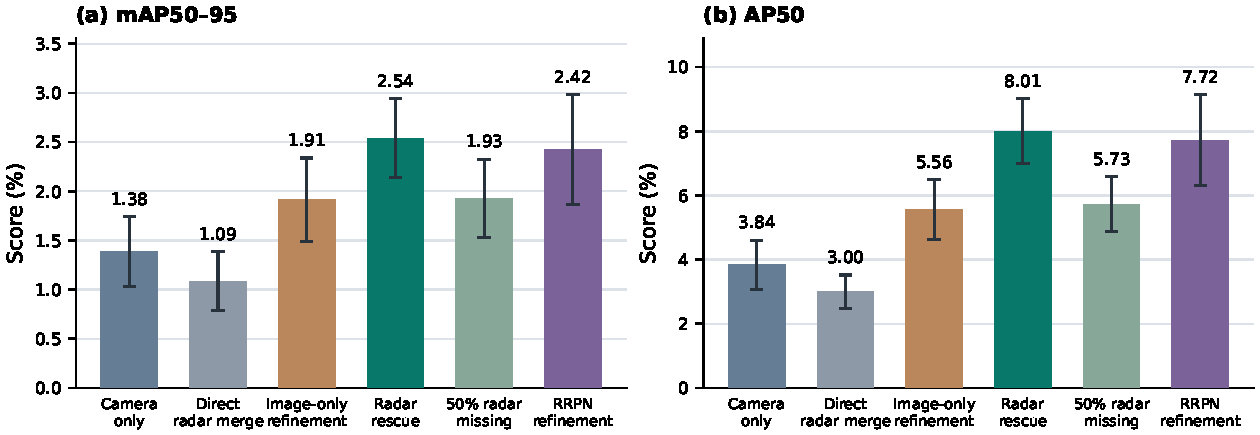
\includegraphics[width=.9\textwidth]{severe_comparison.pdf}
\caption{nuScenes mini 验证集上六种方法在高斯强模糊（$\sigma=4$）下的检测结果。柱高与柱顶标注为三个随机种子的平均值，误差线表示均值上下各一个样本标准差。}\label{fig:diagnostics}
\end{figure*}

\subsection{分类别结果与雷达依赖}
\begin{table}[!t]
\centering\scriptsize
\caption{强模糊下三个种子的分类别平均 AP（\%）}\label{tab:classes}
\setlength{\tabcolsep}{2.2pt}
\begin{tabular}{lrrr}
\toprule
方法 & 汽车 & 行人 & 自行车 \\
\midrule
\ClassRows
\bottomrule
\end{tabular}
\end{table}
\DiagnosticResult{}

直接合并雷达框的 AR100 为 5.13\%，高于纯相机的 3.17\%，但其 mAP50--95 下降到 1.09\%。这一组合可以覆盖更多目标，同时也会引入低质量候选及类别误判。雷达补检同时提高了召回和 AP，表明学习筛选对利用几何候选很重要。AP50 的提高幅度明显大于 AP75，说明有些补检框可以覆盖正确目标，在较严格的重叠标准下仍存在定位误差。三个种子使用同一批验证图像，种子间波动只反映训练随机性。

三个种子的雷达补检分数缩放系数均为 0.02。纯图像精修的对应系数为 0.04、0.02 和 0.04。系数选择使用训练集内的开发场景，验证标签只用于计算本文所报告的指标。

\subsection{边界与结果分析}
图\ref{fig:qualitative}展示两个验证场景在相同人工强模糊条件下的实际预测。上排的纯相机在展示阈值下没有检测框，雷达补检在路面中央给出多个汽车预测框，也留下位置相近的重复框。下排站棚中的密集行人仍有不少未检出。由于单个物体可以产生多个回波，且相邻目标的投影可能重叠，基于 IoU 的抑制并不能消除所有重复框。示例按场景及真值类别数选取，不使用模型结果筛选。完整评价仍使用所有验证帧及低阈值输出。

\begin{figure*}[!t]
\centering
\includegraphics[width=\textwidth]{severe_examples.jpg}
\caption{强模糊条件下的实际推理。按列展示真值、纯相机、纯图像精修与雷达补检。统一显示分数不低于 0.004 的预测。黄色、青色和粉色分别对应汽车、行人、自行车。}\label{fig:qualitative}
\end{figure*}

\subsection{实验范围}
相机主检测器未经强模糊专门微调，纯图像与雷达精修使用相同的模糊增强和精修预算。mini 仅有两个验证场景，自行车框只有 15 个。多个随机种子反映固定划分下的训练波动。下节加入未见场景和独立数据。真实雨雾、低照度及真实运动模糊仍需单独验证。

\section{未见场景与跨数据集验证}
\subsection{固定模型与传感器适配}
两个扩展验证集按 III-A 的划分使用。nuScenes 扩展集逐场景核对了配对帧数与官方元数据，子集由已下载关键帧包的覆盖范围确定。两个验证集均按 $640\times640$ 预处理并施加 $\sigma=4$ 的高斯模糊，三组模型权重和合并分数系数沿用 mini 设置。新增标注只用于评分。

Astyx 提供的回波幅值和径向速度与源模型使用的 RCS 和自车补偿速度定义不同。跨数据集推理时将这两维输入置零，使用经 Astyx 标定投影的雷达位置和深度。Astyx 只报告汽车 AP，nuScenes 仍报告三类 mAP。

\begin{table}[!t]
\centering\scriptsize
\setlength{\tabcolsep}{2pt}
\caption{外部验证三个种子的平均检测 AP（\%）。“—”表示未评价。}\label{tab:expansion}
\begin{tabular}{lrrrr}
\toprule
 & \multicolumn{2}{c}{nuScenes 新场景} & \multicolumn{2}{c}{Astyx 汽车} \\
\cmidrule(lr){2-3}\cmidrule(lr){4-5}
方法 & mAP50--95 & AP50 & AP50--95 & AP50 \\
\midrule
\ExpansionRows
\RrpnExternalRow
\bottomrule
\end{tabular}
\end{table}

\subsection{新增数据的检测结果}
\ExpansionDiscussion{}
\RrpnExternalFinding{}

Astyx 的汽车 AP50--95 为 3.20\%，比纯相机和同型纯图像精修分别高 1.74 和 0.88 个百分点。汽车 AP50 从纯相机的 3.61\% 提高到 10.27\%。在两套新增数据上，移除约一半帧的雷达候选后平均 AP 均下降。该结果检验了冻结补检器在不同场景和雷达数据上的表现。Astyx 只评价汽车，且雷达描述量有两维缺失，因此按数据集分别解读分数。三个种子的同向增益描述固定场景上的结果一致性，样本扩充不能替代真实退化条件的评估。

\section{与 RRPN 候选规则的同条件对比}
\begin{table}[!ht]
\centering\footnotesize
\setlength{\tabcolsep}{3pt}
\caption{nuScenes 强模糊（$\sigma=4$）下的同条件对比，三个种子的 mAP50--95 / AP50（\%）。增量相对纯相机，以百分点计。}\label{tab:comparison}
\begin{tabular}{lrrr}
\toprule
融合方法 & 纯相机 & 融合 & 增量 \\
\midrule
\StrongBlurComparisonRows
\bottomrule
\end{tabular}
\end{table}

表\ref{tab:comparison}在两个 nuScenes 验证集上分别比较，同一验证集内两种方法共享图像、雷达回波、二维标签和评价代码。对照采用 RRPN 公开候选规则及本文的冻结相机与同型精修头。mini 的 81 帧上，本文方法的 mAP50--95 和 AP50 均较高。30 个未见场景的 1191 帧上，RRPN 候选对照的两项指标均较高。两种候选规则的相对排序随验证集变化。

在 mini 上，本文与 RRPN 对照的 mAP50--95 差值仅为 0.12 个百分点，表\ref{tab:seeds}的样本标准差分别为 0.40 和 0.56 个百分点，逐种子结果中两种规则分别取得过较高分数。本文模板平均每帧生成 561.9 个雷达候选，RRPN 为 1685.4 个，较小的候选池减少进入 RoI 精修的框数。未见场景上 RRPN 的 mAP50--95 和 AP50 均较高。本文未测端到端时延，框数用于描述精修工作量。Astyx 的跨数据集结果见表\ref{tab:expansion}。

\section{模块消融实验}
各组沿用相同的冻结相机、训练划分与增强、候选匹配规则及输出抑制设置。五项单模块消融分别去除回波属性、图像 RoI 特征、清晰度特征、边框回归和质量加权。每组在相同的六个训练场景上拟合，在另两个训练场景选择补充框的分数系数，再使用八个场景重训。去除质量加权时，补充分数只使用分类置信度，并在开发集额外搜索较小的系数以适应分数尺度。三个验证集均使用 $\sigma=4$，未见场景和 Astyx 直接复用 mini 拟合结果。

去除回波属性时，精修头中的深度、RCS 和速度置零，候选框及其尺度、位移等模板描述保持一致。去除图像 RoI 特征时同时清零池化的 P3 特征和 RGB 像素，保留清晰度输入。去除边框回归时直接使用未调整的候选框，定位质量目标随之改为候选框的 IoU。为比较候选来源，另设两组成对对照，将雷达描述与模板描述全部置零，两组精修头都仅使用图像特征、清晰度与候选框坐标。

\begin{table}[!ht]
\centering\footnotesize
\setlength{\tabcolsep}{2.5pt}
\caption{三个种子的模块消融均值（\%）。AP 为 AP50--95，nuScenes 对三个类别取平均，Astyx 仅计算汽车。}\label{tab:ablation}
\begin{tabular}{lrrrrrrr}
\toprule
 & \multicolumn{3}{c}{nuScenes mini} & \multicolumn{2}{c}{未见场景} & \multicolumn{2}{c}{Astyx} \\
\cmidrule(lr){2-4}\cmidrule(lr){5-6}\cmidrule(lr){7-8}
设置 & AP & AP50 & AP75 & AP & AP50 & AP & AP50 \\
\midrule
\AblationRows
\bottomrule
\end{tabular}
\end{table}

\AblationMiniFinding{}

\AblationExternalFinding{}

\AblationCandidateFinding{}

\section{结论}
\ConclusionResult{} \ExpansionConclusion{} \RrpnConclusion{} 结论适用于本实验的人工强模糊及前视单帧雷达配置。真实退化与部署性能需要单独评估。

\raggedbottom
\appendices
\section{复现设置与核对方法}
\subsection{场景、初始化和文件}
训练场景为 0061、0553、0655、0757、0796、1077、1094 和 1100。精修头选择系数时留出 0757 和 1094。验证场景为 0103 和 0916。场景编号在 nuScenes 表中统一带 \texttt{scene-} 前缀。精修头使用同种子的相机检查点。生成表格时从三个实际运行中提取 $\sigma=4$ 的验证记录。

\subsection{运行入口和判读}
在服务器项目目录按 README 设置依赖并准备数据。训练精修头时使用与种子匹配的相机检查点。已有实验记录可以直接提取强模糊指标，重新生成表格。重新训练的命令与检查点路径见 README。

\begin{small}
\begin{verbatim}
"$PYTHON_BIN" strong_blur_report.py \
  --extract runs
\end{verbatim}
\end{small}

表格百分比由原始 AP 乘 100，差值使用未四舍五入的 AP。复现包包含每个种子的强模糊指标、LaTeX 源码及运行代码。服务器目录为 \texttt{/home/gyf/}\allowbreak\texttt{camera\_radar\_detection/}，本稿使用 \texttt{runs/rescue\_42}、\texttt{runs/rescue\_43} 和 \texttt{runs/rescue\_44} 的记录。

\subsection{核验输入和输出}
预处理输出 \texttt{manifest.json}，其中记录前视相机关键帧、匹配雷达、场景编号和投影框。首次运行应对照表\ref{tab:data}核验帧数，并检查相机关键帧与雷达点使用同样的缩放、平移坐标。\texttt{results/seed\_42.json} 等记录本稿采用的强模糊条件和对应的精修系数，复核时可直接检查 \texttt{blur\_sigma\_px} 字段。候选覆盖率来自同条件下的独立诊断，保存于 \texttt{results/proposal\_coverage.json}。最终检测表使用学习精修后的输出，与候选框报告的类无关统计口径分开。

从结果文件重建图表时，先读取每种方法在三个种子下的 mAP50--95、AP50 和 AP75，再对同一方法求均值。逐种子表中的离散程度使用样本标准差。雷达缺失结果使用固定缺失帧的原始指标。按相同权重和显示阈值运行推理脚本可以复核图\ref{fig:qualitative}。

\subsection{新增验证数据}
复现包包括 \texttt{prepare\_astyx.py}、\texttt{audit\_expansion.py} 与 \texttt{validate\_expansion.py}。验证程序读取三组 mini 权重并执行推理。\texttt{results/expansion/} 保存新增数据统计、划分核验及逐种子指标。表\ref{tab:expansion} 可用 \texttt{expansion\_tables.py} 重建。原始关键帧包保存在服务器项目的 \texttt{data/expansion/}。

\subsection{RRPN 候选复测}
\texttt{rrpn\_reference.py} 复现公开候选的像素坐标运算，训练与评价命令见 README。\texttt{results/rrpn/} 保存三个种子在两个 nuScenes 验证集上的指标以及候选代码坐标核验记录。\texttt{rrpn\_tables.py} 从这些记录重建表中的复测行。

\subsection{模块消融}
\texttt{module\_ablation.py} 以原始相机检查点和完整、纯图像精修头为起点，拟合并评估消融配置。\texttt{results/ablation/} 保存逐种子、逐数据集的指标和训练内的分数系数搜索记录。\texttt{ablation\_tables.py} 核对参照结果并重建表\ref{tab:ablation}。

\begin{thebibliography}{00}
\bibitem{nuscenes} H. Caesar \emph{et al.}, ``nuScenes: A multimodal dataset for autonomous driving,'' in \emph{Proc. IEEE/CVF CVPR}, 2020, pp. 11621--11631.
\bibitem{nobis} F. Nobis, M. Geisslinger, M. Weber, J. Betz, and M. Lienkamp, ``A deep learning-based radar and camera sensor fusion architecture for object detection,'' in \emph{Proc. Sensor Data Fusion: Trends, Solutions, Applications}, 2019, pp. 1--7.
\bibitem{stacker} L. Stäcker, P. Heidenreich, J. Rambach, and D. Stricker, ``Fusion point pruning for optimized 2D object detection with radar-camera fusion,'' in \emph{Proc. IEEE/CVF WACV}, 2022, pp. 3087--3094.
\bibitem{rrpn} R. Nabati and H. Qi, ``RRPN: Radar region proposal network for object detection in autonomous vehicles,'' in \emph{Proc. IEEE ICIP}, 2019, pp. 3093--3097.
\bibitem{joint} R. Nabati and H. Qi, ``Radar-camera sensor fusion for joint object detection and distance estimation in autonomous vehicles,'' arXiv:2009.08428, 2020.
\bibitem{yangfmcw} Y. Yang, X. Wang, X. Wu, X. Lan, T. Su, and Y. Guo, ``A robust target detection algorithm based on the fusion of frequency-modulated continuous wave radar and a monocular camera,'' \emph{Remote Sens.}, vol. 16, no. 12, Art. no. 2225, 2024.
\bibitem{rcmixer} L. Wang, H. Tuo, Y. Yuan, H. Leung, and Z. Jing, ``RCMixer: Radar-camera fusion based on vision transformer for robust object detection,'' \emph{J. Vis. Commun. Image Represent.}, vol. 107, Art. no. 104367, 2025.
\bibitem{rcbevdet} Z. Lin \emph{et al.}, ``RCBEVDet: Radar-camera fusion in bird's eye view for 3D object detection,'' in \emph{Proc. IEEE/CVF CVPR}, 2024, pp. 14928--14937.
\bibitem{riccardo} Y. Long, A. Kumar, X. Liu, and D. Morris, ``RICCARDO: Radar hit prediction and convolution for camera-radar 3D object detection,'' in \emph{Proc. IEEE/CVF CVPR}, 2025, pp. 22276--22285.
\bibitem{r4det} Z. Xia, Y. Tang, Y. Wang, Z. Wang, and W. Qin, ``R4Det: 4D radar-camera fusion for high-performance 3D object detection,'' in \emph{Proc. IEEE/CVF CVPR}, 2026, pp. 18766--18775.
\bibitem{dongcorruptions} Y. Dong \emph{et al.}, ``Benchmarking robustness of 3D object detection to common corruptions,'' in \emph{Proc. IEEE/CVF CVPR}, 2023, pp. 1022--1032.
\bibitem{wcrd} C. Wang, R. Cheng, H. Yu, X. Gong, and H.-M. Hu, ``Bridging the performance gap of 3D object detection in adverse weather conditions via camera-radar distillation,'' \emph{Displays}, vol. 92, Art. no. 103320, 2026.
\bibitem{astyx} Astyx GmbH, ``Astyx HiRes2019 dataset,'' 2019. Data archive: \texttt{github.com/under-the-radar/}\allowbreak\texttt{radar\_dataset\_astyx}.
\bibitem{yolo} Ultralytics, ``Ultralytics YOLO11,'' official model documentation. \texttt{docs.ultralytics.com/models/yolo11/}.
\bibitem{coco} T.-Y. Lin \emph{et al.}, ``Microsoft COCO: Common objects in context,'' in \emph{Proc. ECCV}, 2014, pp. 740--755.
\end{thebibliography}
\end{document}
